\chapter{Virtuelle LANs}

Virtuelle Netze oder auch virtuelle local area networks (VLAN) ermöglichen es, bestehende physische LANs in logische Abschnitte zu Unterteilen, oder auch mehrere physische Netzabschnitte virtuell zu verbinden. VLANs werden mithilfe von Switches gebildet. Switche sind Netzwerkkomponenten, welche die Schichten eins und zwei des Internetprotokollstapels (vgl. Anhang \ref{A1}) implementieren, sie bilden heute die Zentralen Netzknoten in (lokalen) Netzwerken \cite{zisler2018computer}. 
Durch das Verwenden von VLANs können Kosten gespart werden, wenn mehrere Netzwerke durch weniger  Hardware realisiert werden können. Virtuelle Netze sind flexibler als physische Netze. In größeren Netzwerken kommt außerdem die Tatsache zum tragen, dass die Broadcastdomänen durch die logische segmentierung verkleinert werden, da Broadcasts die innerhalb ihres VLANs bleiben.

%nutzen hinzufügen

\section{Funktionsweise}

% portbasiertes und tagged Vlan

Es gibt zwei Arten von Vlans, das portbasierte und das \emph{tagged VLAN}. 
Bei dem in Abbildung \ref{vlanport} dargestellten portbasiertem VLAN, wir jeder Port eines Switches einem VLAN zugewiesen. Soll nun eine Kommunikation zwischen den Geräten, die a VLAN A angeschlossen sind und jenen aus VLAN B stattfinden, müssen jeweils ein Port aus VLAN A mit einem aus VLAN B per Kabel verbunden werden und ein Router müsste zwischen diesen Netzen vermitteln\cite{cisco14rout}.  


\begin{figure}[h]
\centering
	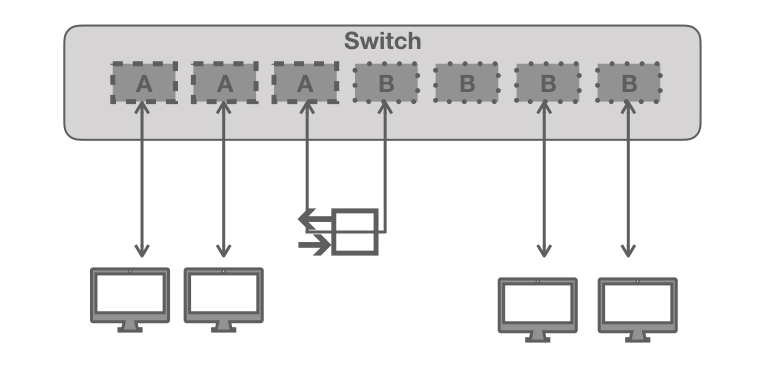
\includegraphics[width=0.8\linewidth, height= 6cm]{vlan.001.jpeg}
	\caption{Portbasiertes VLAN}
	\label{vlanport}
\end{figure}


Das in Abbildung \ref{vlanpak} gezeigte \emph{tagged} VLAN ermöglicht es, dass ein Port auch mehreren VLANs zugeordnet werden kann. Bei  diese Art des virtuellen Netzes können VLANs, die über  Switche verteilt sind mit nur einem Kabel verbunden werden, wofür sonst je VLAN ein Kabel verwendet werden müssten. Die Verbindung zwischen zwei Switches über die mehrere VLANs laufen wird Trunk genannt \cite{cisco14rout}. 

\begin{figure}[h]
\centering
	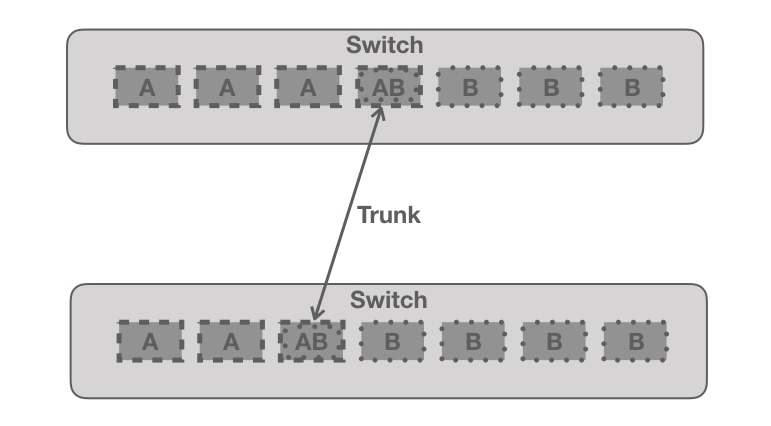
\includegraphics[width=0.8\linewidth,height=6cm]{vlan.002.jpeg}
	\caption{Tagged VLAN}
	\label{vlanpak}
\end{figure} 

Die Zugehörigkeit der Pakete zu einem VLAN wird über einen VLAN-Tag nach dem Standard  IEEE 802.1Q am Ehternet-Frame gekennzeichnet.\\

Es wird zwischen statischen und dynamischen VLAN Implementierungen unterschieden. Beim statischen VLAN wird 
\\

Bei der Auslieferung sind in einem Switch alle Ports demselben \emph{default} VLAN zugeordnet. Wenn der Switch in Betrieb genommen wird sollten einige, im Folgenden erläuterte,  Punkte beachtet werden. Alle Ports die nicht verwendet werden sollten ein eigenes VLAN bekommen, das ins leere läuft. Bei der Verwendung von Trunks zwischen Switches gibt es ein \emph{native} VLAN über das Pakete gesendet werden, die keinen Tag haben. Solche Pakete können von Switches stammen, die kein Protokoll mit tagging unterstützen. Dieses native VLAN sollte ein eigenes VLAN sein, um hier keine Angriffspunkte zu bieten. Außerdem sollte ein gesondertes \emph{management} VLAN erstellt werden über das Zugriff auf die Konfiguration des  Switches besteht. 




\section{VLAN und Sicherheit}

\glqq Entgegen den Aussagen einiger Hersteller muss berücksichtigt werden, dass VLANs nicht entwickelt wurden, um Sicherheitsanforderungen bei der Trennung von Netzen zu erfüllen.\grqq (Bundesamt für Siherheit in der Informationstechnik: \cite{bsiswitch}).\\

Trotzdem bringen VLANs gerade für kleinere Unternehmen einige Vorteile in der Datensicherheit, da sie, richtig konfiguriert, zumindest eine zusätzliche Hürde für Angreifer darstellen.

Zunächst sollen mögliche Angriffe auf virtuelle LANs vorgestellt werden.

 \subsubsection{VLAN Hopping}
  Bein VLAN Hopping befindet sich ein Angreifer in einem VLAN und versucht in ein anderes VLAN zu gelangen\cite{alabady2008design}. 
  Eine Möglichkeit hierzu ist das \emph{double tagging}. Befindet sich der Angreifer in dem Vlan das als natives VLAN konfiguriert wurde kann er ein Ethernet Frame mit zwei Tags abschicken, den des nativen VLANs und einem weiteren des Ziel VLANs. Das Switch entfernt dann den ersten Tag und leitet den Frame weiter, ohne ein neues Tag hinzuzufügen, da die bei dem nativen VLAN nicht benötigt wird. Gelangt das Paket nun über einen Trunk zu einem weiteren Switch sieht dieser nur den zweiten Tag und leitet den Frame an das Opfer-VLAN weiter.
  Um diese Art des Angriffs zu Verhindern sollten keine Geräte an das native VLAN angeschlossen werden \cite{cisco14rout}.\\
  
  
  
 Eine weitere Form des VLAN Hoppings ist das \emph{switch spoofing}, welches ausnutzt, dass einige Switches automatisch erkennen, wenn ein anderer Switch versucht eine Trunk Verbindung aufzubauen und diese erwidern. Ein Angreifer kann vorgeben ein anderes Switch zu sein und somit erreichen, dass ein switch mit ihm eine Trunk-Verbindung eingeht, so bekommt der Angreifer die Kommunikation aller VLAN gesendet. 
 
 Die Funktion des Automatischen Trunkings sollte für alle nicht-Trunk-Ports ausgeschaltet werden um switch spoofing zu verhindern \cite{cisco14rout}. 
 
  
   
 
 


